\chapter{Human Body Estimation}
In this chapter, I will explain how I managed to estimate the parametric model of the patient exploiting visual information.

\section{SMPL models family}
For the body shape and pose, there is a well known model called SMPL (Skinned Multi-Person Linear Model) \cite{SMPL:2015} which is a realistic 3D model of the human body that is based on skinning and blend shapes. SMPL is learned from thousands of 3D body scans. SMPL model pose is described by 23 body joints together with body position and orientation called $\vec{\theta}$, while the body shape is described by 10 parameters called $\vec{\beta}$. Each $\theta_i, i \in [1,21] $ represents the 3D orientation of a human joint with respect to its kinematic parent. The kinematic tree is expressed as a connectivity map that connect each joint to its child, as shown in \autoref{fig:human-body-estimation:kin_tree}.
\begin{figure}[h]
    \centering
    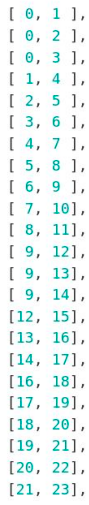
\includegraphics[width=0.07\linewidth]{images/kinematic_tree.png}
    \caption{The SMPL kinematic tree}
    \label{fig:human-body-estimation:kin_tree}
\end{figure}
Orientations are represented by rotation vectors and can be converted to rotation matrices using the Rodriguez formula. % The inference of the SMPL is the prediction of the joint location thanks to a joint regressor, then the computation of the blend skinning of the model starting from the T-pose and finelly the .%
Since the model is linear, the inference time is fast.
There exist multiple variants of this model:
\begin{itemize}
    \item SMPL-H\cite{MANO:SIGGRAPHASIA:2017} is the extended version of SMPL that accounts also for hands position. It leverages on 21 body joints from the SMPL model, replacing the two additional joints related to the hand position with 15 additional joints for each hand.
    \item SMPLX\cite{SMPL-X:2019} (SMPL eXpressive) is the extended version of SMPL-H which accounts also for the face expressions. The total number of joints is 54 which includes joints for the neck, jaw, eyeballs, and fingers. 
\end{itemize}
The difference between SMPL and SMPLX is show in \autoref{fig:human-body-estimation:smpl}.
\begin{figure}[h]
    \centering
    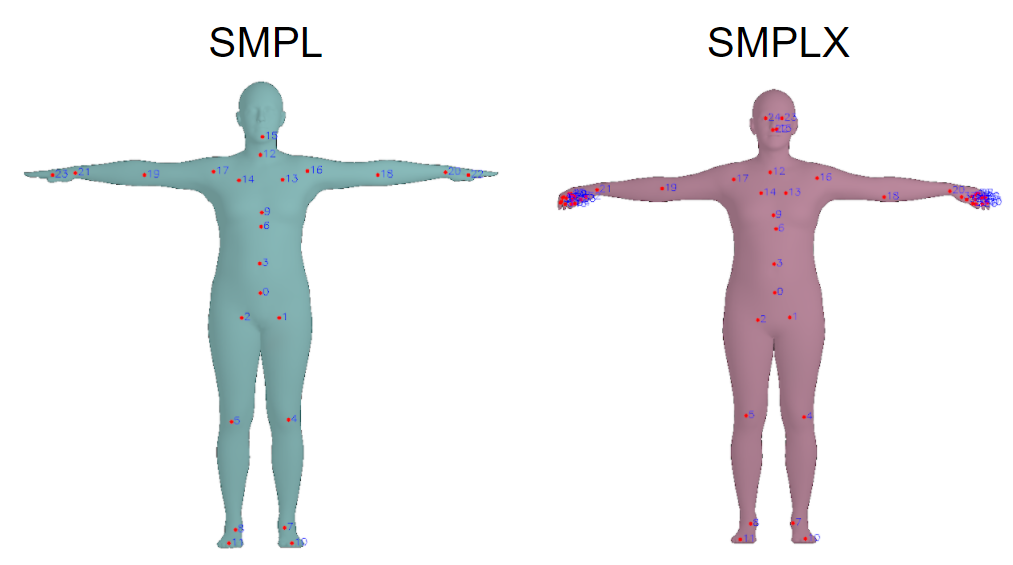
\includegraphics[width=0.7\linewidth]{images/smpl.png}
    \caption{The comparison of the number and location of joints for SMPL and SMPLX}
    \label{fig:human-body-estimation:smpl}
\end{figure}
These more recent extensions of SMPL can be used in tasks where knowing the exact hand configuration is crucial or when the facial expression information can be exploited in some way. In my opinion, SMPL-H and SMPLX will be soon introduced in different human-robot collaboration scenarios. Since for RLU hands and facial expressions were not included in the logic of my thesis I took the SMPL for modelling the patient state.

\section{Human body pose estimation}
As already mentioned in the previous section, the SMPL model is composed by $\vec{\theta}$ and $\vec{\beta}$. It is possible to animate a SMPL model in real-time if $\vec{\beta}$ does not need to be optimized, updating just the $\vec{\theta}$ parameters of the model.
For this purpose I used a \verb|ZED2| stereo camera which integrates an AI body tracking module\cite{zed_body_tracking} based on the depth and RGB image measured by the sensor itself. The body tracking module provides different skeleton models. I chose the one more similar to SMPL, which is also the most informative, since it is the one with the highest number of keypoints (38). A figure showing the pose of the keypoints is reported in \autoref{fig:human-body-estimation:zed_kp}.
\begin{figure}[H]
    \centering
    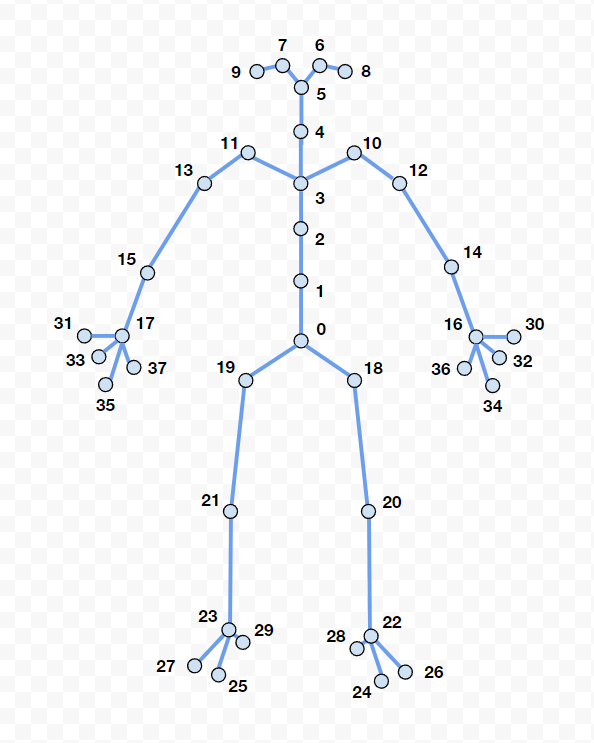
\includegraphics[width=0.5\linewidth]{images/zed_kp.png}
    \caption{BODY38 model provided by the ZED SDK}
    \label{fig:human-body-estimation:zed_kp}
\end{figure}
Comparing \autoref{fig:human-body-estimation:smpl} and \autoref{fig:human-body-estimation:zed_kp} it is easy to notice that the joint location is similar between the two models, so it was straight forward to compute the right input for the SMPL model for the real time animation. Since the \verb|ZED| AI module already provides the local orientation of each joints with respect to its parent in the kinematic tree (which is the same of the SMPL), it was sufficient to convert from the quaternion notation for the orientation to the rotation vector notation.

\section{Human body shape estimation}
\label{section:human-body-shape-estimation}
Given that this master's thesis aims to address the problem of the physical variability between patients in RLU, $\vec{\beta} \in \mathbb{R}^{10}$ is a crucial parameter to be considered since it affects the rib cage dimension and position. An external source of information is required in order to evaluate a metric for the shape parameters optimization. I decided to use the same exteroceptive sensor used for the pose estimation procedure: the \verb|ZED2|. Therefore, I retrieved the raw point cloud of the scene. 

\section{Human Instance Segmentation with YOLOv8}
Since I needed an intelligent way of ignoring points not belonging to the human, I exploited YOLOv8 segmentation neural network from Ultralytics in order to detect which image pixel belongs to the patient. YOLOv8 segmentation is an advanced computer vision model that combines object detection with instance segmentation. Ultralytics provides different models for the instance segmentation of 80 different classes. 
When applied to human body segmentation, it not only identifies humans in an image but also generates a precise mask outlining the shape and boundaries of the body. This is achieved through pixel-level predictions, allowing the model to differentiate the human body from the background and other objects. YOLOv8's segmentation capabilities are highly efficient, making it suitable for real-time applications like pose estimation, augmented reality, and medical imaging.  

\section{Point Cloud Filtering using YOLOv8Seg Mask}
The mask computed by YOLO is represented by the vertices of a polygon. I converted it to a bit mask matrix through the \verb|fillPoly| of \verb|opencv| having 1 or 0 for each pixel of the original image. The resulting image is then used to decide which points of the point cloud to discard. Moreover, I exploited the bounding box provided by YOLO in addition to the mask to limit the amount of computation needed to filter the point cloud. To be more explicit, I restricted the double nested loop over the image pixels to the bounding box instead of the full image. The resulting point cloud is illustrated in \autoref{fig:human-body-estimation:yolo-seg}


\begin{figure}[h]
    \centering
    \subfloat[\centering RGB Image from the left sensor of the stereo camera with the yolo segmentation mask colored in red]{{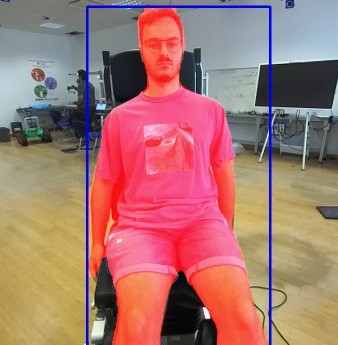
\includegraphics[width=5cm]{images/body_estimation/yolo_seg.jpg} }}%
    \qquad
    \subfloat[\centering Point cloud obtained removing the points relative to the pixels filtered by the mask]{{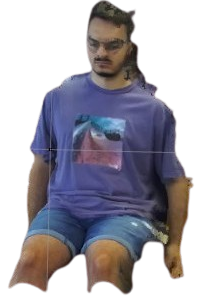
\includegraphics[width=3cm]{images/body_estimation/point_cloud.png} }}%
    \caption{}%
    \label{fig:human-body-estimation:yolo-seg}%
\end{figure}

\section{SKEL, a biomechanical model}
SKEL\cite{keller2023skel} is a biomechanical skeleton model that maps the SMPL skinned model to its anatomical skeleton. The new model differs from the existing SMPL model in several key ways:
\begin{itemize}
    \item Anatomical accuracy: In comparison to SMPL, SKEL offers more precise joint placements and anatomically correct bone orientations. It includes biomechanical factors, like better knee alignment and arm supination, that enable a more accurate depiction of human anatomy.
    \item Posture parameters: SKEL is more effective in regressing precise anatomical joints from video data because it has fewer posture parameters (46), as opposed to SMPL's (72). Applications in computer vision and biomechanics benefit from this reduction in parameters.
    \item Biomechanical features: SKEL incorporates a biomechanical shoulder blade that enables for more realistic movement in place of the SMPL's approximation shoulder structure. Additionally, it simulates how the ulna and radius bones move in the forearm pronation and supination, which constitute a major advancement above the SMPL's basic rotation around the elbow.
    \item Integration of skin and skeleton: SKEL enables direct animation of both components by concurrently rigging the skin and skeleton meshes with the same pose parameters. For this reason, SKEL can inherit the pose and shape directly from SMPL.
    \item Data utilization: To improve the accuracy of the skeletal structure and joint placements, SKEL makes use of the BioAMASS dataset, which integrates motion capture data with anatomical information. In comparison, SMPL does not include such comprehensive biomechanical data.
\end{itemize}

Compared to the SMPL framework, SKEL represents a substantial leap in producing 3D human models that are more lifelike and anatomically precise. An illustrative image of SKEL can be observed in \autoref{fig:human-body-estimation:skel} 
\begin{figure}[H]
    \centering   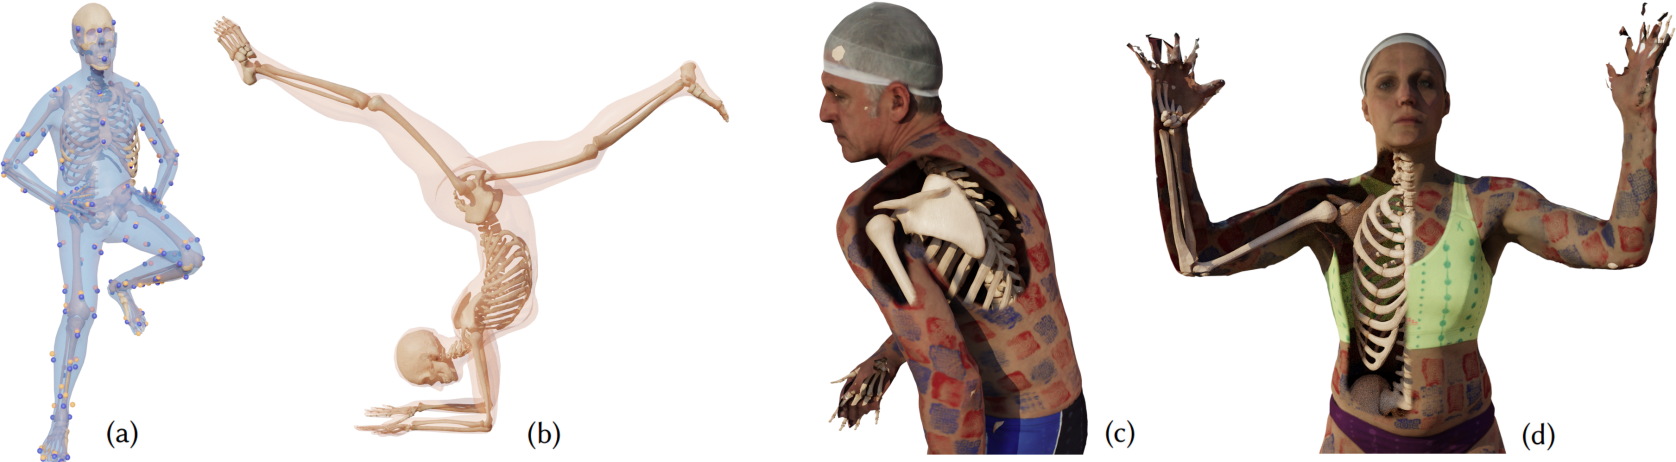
\includegraphics[width=0.7\linewidth]{images/skel.png}
    \caption{An image taken from the SKEL paper, as we can see in the images on the left, both the skin and the skeleton are present in the output of the SKEL model}
    \label{fig:human-body-estimation:skel}
\end{figure}
\section{SKEL Fitting from SMPL}
Since I computed the SMPL from the patient state in \autoref{section:human-body-shape-estimation}, the next step was to compute the skeleton inside the SMPL mesh. Since SKEL has the same surface mesh topology and shape parameters $\vec{\beta}$ as SMPL, it can be directly fit to existing SMPL meshes by optimizing its pose parameters to minimize the vertex-to-vertex
error between the SMPL skin and the SKEL skin. The alignment is avoid local minima by aligning the model in this order:
\begin{enumerate}
\item Align pelvis
\item Align forearm and thighs
\item Align elbows and knees 
\item Align hands, feet, and neck
\end{enumerate}
The order is the same of the kinematic tree since each joint position depends on its predecessor. In order to locally optimize some particular joints, it is sufficient to mask the not relevant contributions in the loss computation. The loss used for the optimization were:
\begin{itemize}
    \item Pose loss: The loss between the joint position of SMPL and the one of SKEL
    \item Vertex loss: Since the skin mesh of SMPL is the same as SKEL, it is possible to compute vertex-wise displacement
    \item Scapula loss: loss added to regularize the scapula fitting avoiding large values, implemented with masking on non-relevant joints
    \item Spine loss: loss added to regularize the spine fitting avoiding large values, implemented with masking on non-relevant joints
\end{itemize}
\TODO add formula
\section{Modelling the rib cage projection on the skin}
Once the SKEL model is computed from the SMPL retrieved from the point cloud, we need to understand where it is located during the robot interaction with the skin. Different geometrical intuition and approximation can be used to estimate how the rib cage is projected on the skin. My first idea was to radially project the skeleton mesh vertices to the skin. The result was poor, especially for ribs far from the projection centre. I then switched to cylindrical projection, considering the cylinder axis parallel to the backbone. The results were qualitatively more realistic than the one produced by the spherical projection. The projection was implemented using ray casting algorithm provided by \verb|Open3d| that finds the 3D intersection point of a ray to a mesh. A visual comparison between radial and cylindrical projection is shown in \autoref{fig:human-body-estimation:skeleton-projection}.
\begin{figure}[H]
     \centering
     \begin{subfigure}[b]{0.3\textwidth}
         \centering
        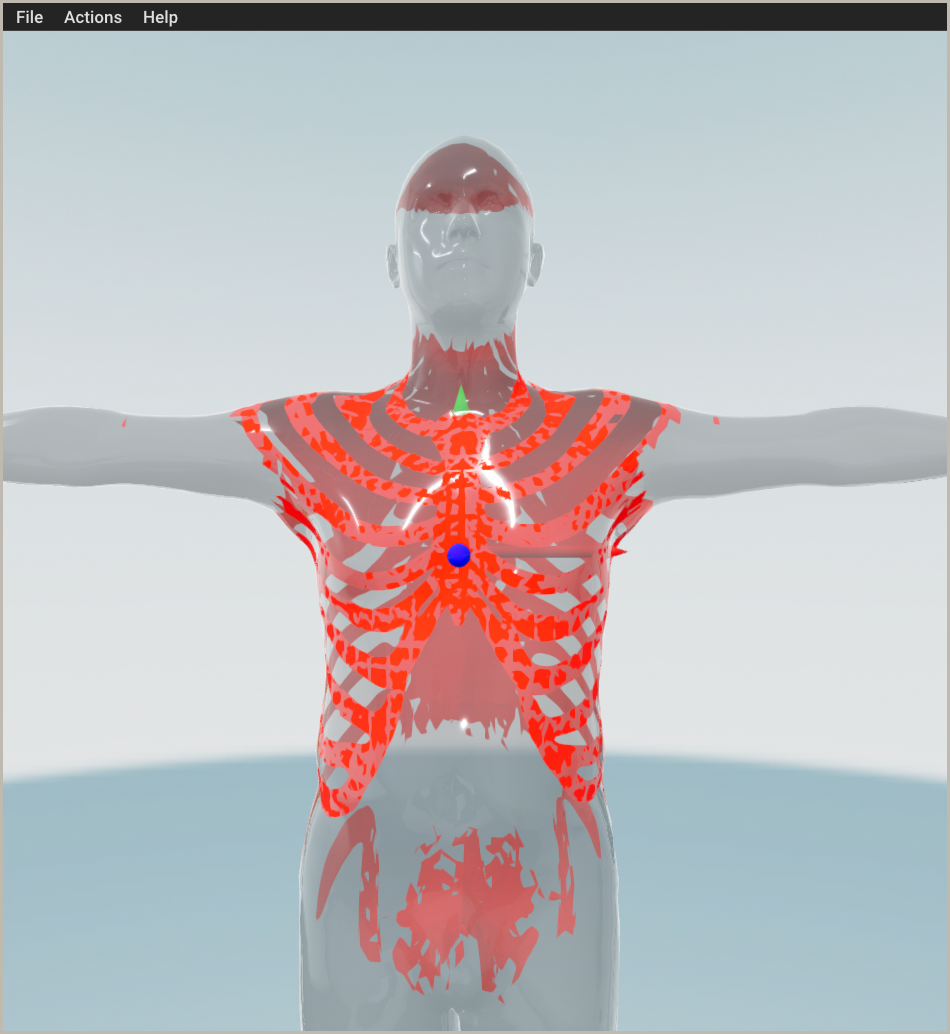
\includegraphics[width=\textwidth]{images/body_estimation/radially_proj.png}
         \caption{}
         \label{}
     \end{subfigure}
     \hfill
     \begin{subfigure}[b]{0.3\textwidth}
         \centering
         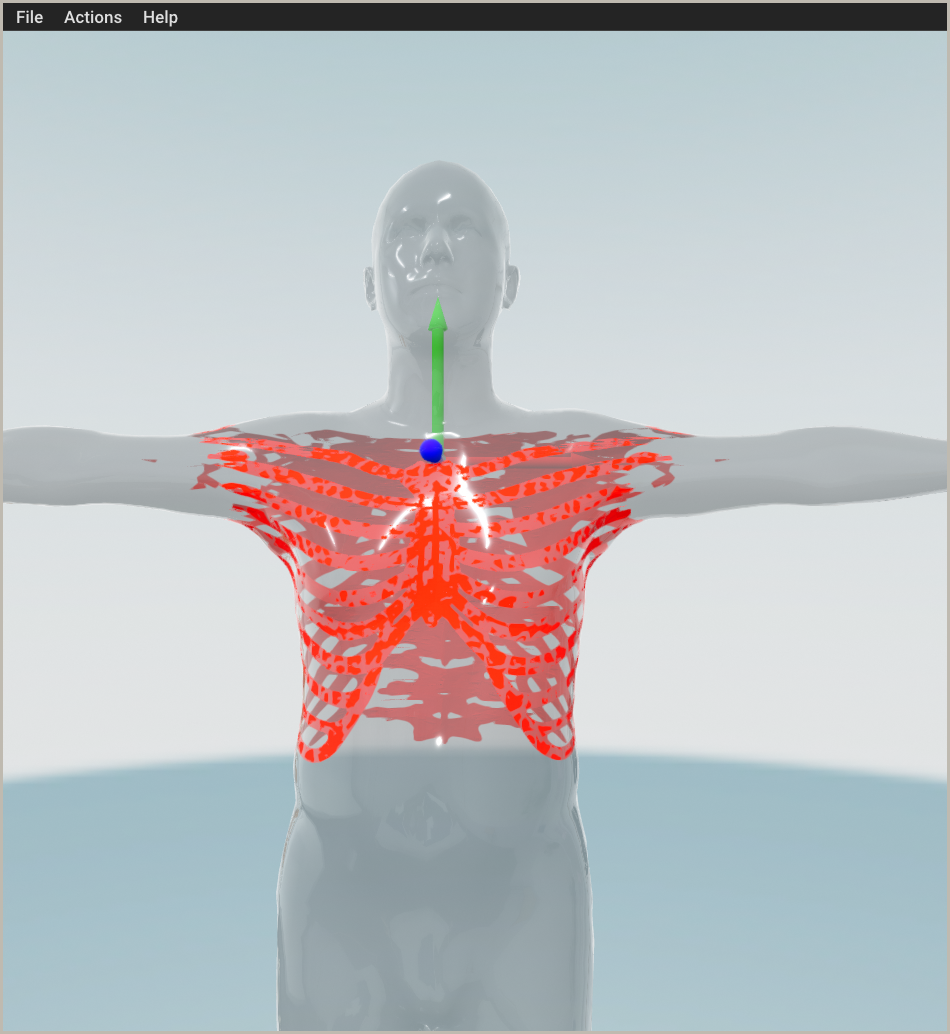
\includegraphics[width=\textwidth]{images/body_estimation/cylindrical_proj.png}
         \caption{}
         \label{}
     \end{subfigure}
\caption{Comparison between the two projection methods tested: on the left the radial projection, on the right the cylindrical projection}
\label{fig:human-body-estimation:skeleton-projection}
\end{figure}

Since each vertex is projected on the skin, the result is a point cloud. We can reconstruct a mesh from the projection connecting each vertex to his adjacent vertices in the original rib cage mesh.
The result of such operation is shown in \autoref{fig:human-body-estimation:projection_reconstruction}. As we can notice, the ribs are reconstructed correctly.
%% TODO parlare dell'ottimizzazione con loss functions ecc
\begin{figure}[H]
    \centering   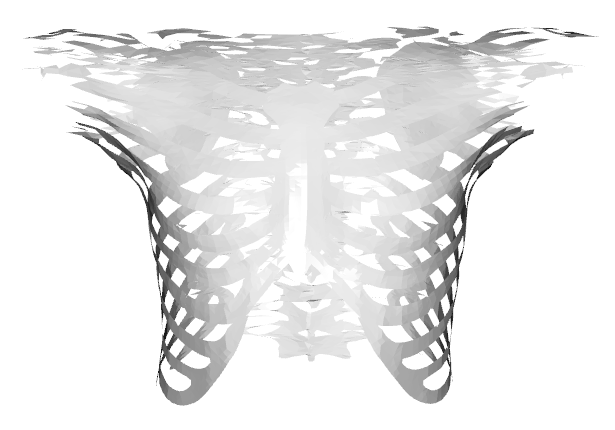
\includegraphics[width=0.7\linewidth]{images/body_estimation/rib_cage_proj.png}
    \caption{The resultant mesh obtained from the point cloud retrieved by the cylindrical projection of the rib cage original mesh.}
    \label{fig:human-body-estimation:projection_reconstruction}
\end{figure}
The idea is to create a virtual fixture that guide the physician towards the intercostal area, exploiting the semantic knowledge expressed by the SKEL model to compensate the lacks of the teleoperation.